\documentclass[conference]{IEEEtran}
\usepackage{times}

% numbers option provides compact numerical references in the text. 
\usepackage[numbers]{natbib}
\usepackage{multicol}
\usepackage[bookmarks=true]{hyperref}
\usepackage{graphicx}
\usepackage{amsmath,amsfonts,amssymb}
\usepackage{hyperref}

\graphicspath{ {./graphics/} }

\pdfinfo{
   /Author (Mingyo Seo)
   /Title  (Robots: Our new overlords)
   /CreationDate (D:20101201120000)
   /Subject (Robots)
   /Keywords (Robots;Overlords)
}

\begin{document}

% paper title
\title{CS391L HW4: Gaussian Process}

% You will get a Paper-ID when submitting a pdf file to the conference system
\author{Mingyo Seo}

\author{\authorblockN{Mingyo Seo}
\authorblockA{
UT EID: ms84662\\
Email: mingyo@utexas.edu}}



\maketitle

\IEEEpeerreviewmaketitle

\begin{abstract}
In this assignment, an overview of Gaussian processes (GP) is presented and is applied to estimate a trajectory from human motions.
We used a dataset of 5 different iterations of same motion and mixed signals to generate a single trajectory.
In particular, we used an exponated RBF kernel for the trajectory processing.
The regression was implemented by the gradient descent algorithm to maximize the negative log likelihood function, which outputs the optimal kernal hyperparameters.
We also compared the use of a single global GP and a set of GP's fit to local data, and studied how the local GP's hyperparameters change.

\end{abstract}

\section{Introduction} % Introduce your problem and the overall plan for approaching your problem

The problem of estimate a trajectory from multiple demonstration can be applied to many areas.
In this paper, in particular, we implemented a Gaussian process(GP) model to estimate a trajectory from human demonstration. 
GP is one of statistical parameter-free models.
By using a GP model, we can predict and estimate a likelihood at any given dataset.
We can consider a GP as an multi-dimensional Gaussian Probability density function (PDF).
A GP is characterized by a set of the mean and variance functions.
By sampling an finite or infinite dimensional PDF, we can regress the mean and variance functions, which is formulized as,
\begin{equation}
\begin{aligned}
    f \in \mathcal{N}(\mu(\boldsymbol{x}),V(\boldsymbol{x}))\ \text{sampled from PDF},\\
    \text{where} \quad \mu \in R^n,\ V\in R^n\times R^n.
\end{aligned}
\end{equation}
For the implementation of GP, we used a mixed motion demonstration data from multiple datasets to estimate a motion trajcetory.

The answers to the HW4 questions are included in the following sections.
\begin{itemize}
\item Fig. \ref{fig:signal}: Visualization of base, mixed, recovered signals
\item Fig. \ref{fig:basic_test}, \ref{fig:basic_abs_test}, \ref{fig:batch_abs_test}, \ref{fig:eta_abs_test}, \ref{fig:sample_abs_test}: Correlation between source and recovered signals
\end{itemize}



\section{Method}
\label{sec:method}

\subsection{Finite Gaussian Process}
We assume that the prior distribution follows a Gaussian distribution of mean($m_f$) and identity Co-variance matrix($K_{ff}$), represented as,
\begin{equation}
\begin{aligned}
    &\quad f(\boldsymbol{x})\ \sim \ GP(m(x),\kappa(x,x')) \Leftrightarrow f \in \mathcal{N}(m_f,K_{ff}),
\end{aligned}
\end{equation}
where
\begin{equation}
\begin{aligned}
    &m(x) = \mathbb{E}[f(x)]\\
    &\kappa(x,x') = \mathbb{E}[(f(x)-m(x))(f(x')-m(x'))].
\end{aligned}
\end{equation}
Thus, we can update the posterior from a data $(X, y)$
By using Bayes' theorem, the GP is represented as,\\
\begin{equation}
\begin{aligned}
    &P(f|y)\\ 
    &\quad = \mathcal{N}(K_{fy}^TK_{yy}^{-1}(y-m_y) +m_f, K_{ff}-K_{fy}^TK_{yy}^{-1}K_{fy}^T).
\end{aligned}
\end{equation}
The above formulas exist in an infinite dimensional space. 

To apply the form of an infinite GP into a finite data set, we reformulate the GP formulation and use a Kernel function to calculate the co-variance matrix. 
If the optimal GP of the finite data set $(X,y)$ is given by $f$, then predictions for new data $X_*$ given by $f_*$ are given as,
\begin{equation}
\begin{aligned}
    \begin{bmatrix}
    f\\
    f_*
    \end{bmatrix} = \mathcal{N}\left( 0, \begin{bmatrix}
    K(X,X)\    K(X,X_*)\\
    K(X_*,X)\    K(X_*,X_*)
     \end{bmatrix}    
    \right)
    \label{eq:Ensemble}
\end{aligned}
\end{equation}
Instead of sampling multiple $f_*$ from the ensemble of equation \ref{eq:Ensemble}, we can condition our prior of $f$ for $(X,y)$. 
If there is no noise in the observed output $y$, then the best solution is $f=y$, and
\begin{equation}
\begin{aligned}
    f_*|X_*,X,f & \\
    \sim \mathcal{N} (& K(X_*,X)K(X,X)^{-1}f, \\
    & K(X_*,X_*)- K(X_*,X)K(X,X)^{-1}K(X,X_*)) 
    \label{eq:fstar}
\end{aligned}
\end{equation}
In particular, we use an exponated RBF kernel to calculate the co-variance matrix $K$ and Gaussian noise to estimate raw data errors, given as
\begin{equation}
\begin{aligned}
    &y(u) = f(u) + \epsilon\\
    &k(u_i,u_j) = e^{\sigma_f}e^{\left(\frac{1}{2}e^{\sigma_l}||u_i-u_j||^2\right)} \\
    &q(u_i,u_j) = k(u_i,u_j) + e^{\sigma_n}\delta_{ij},
    \label{eq:Kernel with noise}
\end{aligned}
\end{equation}
where $\epsilon \sim \mathcal{N}(0,e^{\sigma_n}).$
This also can be written as, 
\begin{equation}
\begin{aligned}
Q(X,X) = K(X,X) + e^{\sigma_n}I_{n\times n}.
\end{aligned}
\end{equation}
Then, we can estimate $f_*$ for new values $X_*$ using equation \ref{eq:fstar}, as
\begin{equation}
\begin{aligned}
    &\Bar{f_*} = K(X_*,X)K(X,X)^{-1}y\\
    &\mathbb{V}[f_*] = K(X_*,X_*) - K(X_*,X)Q(X,X)^{-1}K(X,X_*),
\end{aligned}
\end{equation}
where $K(X_*,X) = \left[K(X,X_*)\right]^T$.
The variance at each $x_*$ is given by the diagonal elements of $\mathbb{V}[f_*]$. 
The standard deviations from these values can be used to compute the 95\% confidence interval at each $x_*$.
Also, from $f_*$, we can also calculate the expectation and variance of the observations $y_*$. Since adding white noise does not change mean observation, the mean is given as,
\begin{equation}
\begin{aligned}
    \Bar{y_*} = \Bar{f_*}.
\end{aligned}
\end{equation}
The variance is given as
\begin{equation}
\begin{aligned}
	\mathbb{V}[y_*] = Q(X_*,X_*) - K(X_*,X)Q(X,X)^{-1}K(X,X_*).
\end{aligned}
\end{equation}


\subsection{GP Hyperparameter regression}

A regression on the hyper-parameters, $\sigma = [\sigma_f,\sigma_l,\sigma_n]$ obtains the optimal GP over the given data. 
Consider the log-likelihood function, given as 
\begin{equation}
\begin{aligned}
    log P(y|x,\sigma) = -\frac{1}{2}y^TQ^{-1}y - -\frac{1}{2}log(det(Q)) - \frac{n}{2}log(2\pi)
     \label{eq:logP}
\end{aligned}
\end{equation}
The GP regression can be processed by maximizing the log-likelihood function \cite{bishop}, as 
\begin{equation}
\begin{aligned}
	\sigma_{i+1} = \sigma_{i} + \eta\cdot
	\left[ {\nabla}_\sigma (log P) \right]_{\sigma_i}.
	\label{eq:gradient ascent}
\end{aligned}
\end{equation}
Here, $\eta$ is the vector learning rate.
Then, the gradient of the $logP$ function is given by:
\begin{equation}
\begin{aligned}
    {\nabla}_\sigma(log P) = -\frac{1}{2}y^T\frac{\partial Q^{-1}}{\partial \Vec{\sigma}}y - -\frac{1}{2}\frac{\partial log(|Q|)}{\partial \Vec{\sigma}},
\end{aligned}
\end{equation}
where
\begin{equation}
\begin{aligned}
    &\frac{\partial log(|Q|)}{\partial {\sigma}} = trace\left( Q^{-1}\frac{\partial Q}{\partial {\sigma}}\right)\\
    &\frac{\partial Q^{-1}}{\partial {\sigma}} = -Q^{-1} \frac{\partial Q}{\partial {\sigma}} Q^{-1},
\end{aligned}
\end{equation}    
and the partial differentials are given as,
\begin{equation}
\begin{aligned}
    &\frac{\partial Q_{ij}}{\partial \sigma_f} = K_{ij}\\
    &\frac{\partial Q_{ij}}{\partial \sigma_l} = K_{ij}\times \left(-\frac{1}{2}e^{\sigma_l}||x_i-x_j||^2 \right)\\
    &\frac{\partial Q}{\partial \sigma_n} = e^{\sigma_l}I.
\end{aligned}
\end{equation}

\section{Results} % Describe the methods you intend to apply to solve the given problem


a starting point of $\Vec{\sigma}_0 = [-1,-8,-8]$ with $\eta=10^{-3}$ was stable for almost all data and markers in the experiment. The gradient ascent was stopped when the magnitude of the gradient fell below a tolerance value (tol), i.e. $||\Vec{\nabla}_\sigma(Q)||_1\ <\ tol$. A tolerance of 1 was found to best based on computation time and goodness of fit.

There is a strong negative correlation between the hyperparameters $sigma_f$ and $sigma_l$.
When multiple dataset were mixed together to produce noisy data, then this negative correlation was not as apparent.


The ICA implementation of using MLE and gradient descent described in Section \ref{sec:method} is implemented under the environment of python scripts (3.8.5) and numpy (1.17.5). The model is trained and evaluated by the sound dataset from the class website \cite{cs391}. We used random mixes of $n=3$ source signals from the dataset and initialized $W_0$ to be random matrices where each entry in $[0, 1]$.


\subsection{Signal restoration}

In the assignment, the performance of the model is evaluated by correlation between original signals and recovered signals. We paired a restored signal with the orignal signal that has the largest magnitude of correlation. In the experiment, we used $n=3$, $m=3$, $\eta=0.01$, $t=16$ and the maximum interation $k_{\text{max}} = 5000$.

The source signals, the mixed signals, and the restored signals after $k_{\text{max}}$ are presented in Fig. \ref{fig:signal}.
The plot of correlation between the source signals and the restored signals is presented in Fig. \ref{fig:basic_test}.

Due to the semi-symmetric nature of waves, the largest correlation of Signal \#3 became negative, which implies that the extracted signal has the opposite phase of the original source signals. We use the plot of absolute correlation as Fig. \ref{fig:basic_abs_test} and find that correlation increase as an iteration number increases. For readability, we use absolute correlation for analyzing the effectiveness of the model in the following subchapters. Also, we can find that each source signal matches with the paired signals, which implies the ICA model successfully extracts original signals from mixed signals.

\begin{figure}[!t]
	\centering
	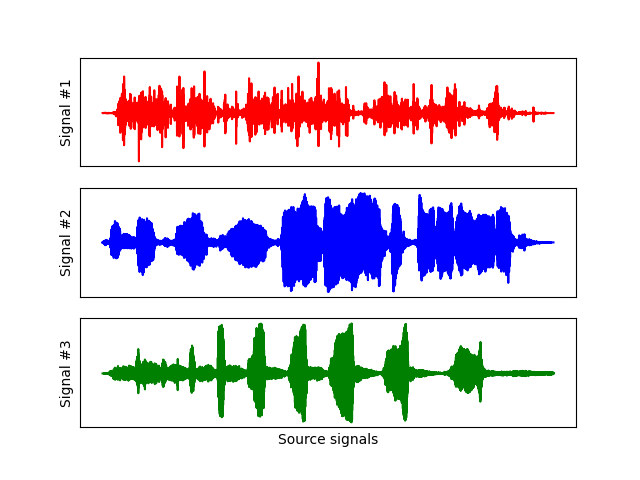
\includegraphics[width=3.6in]{original.png}	
	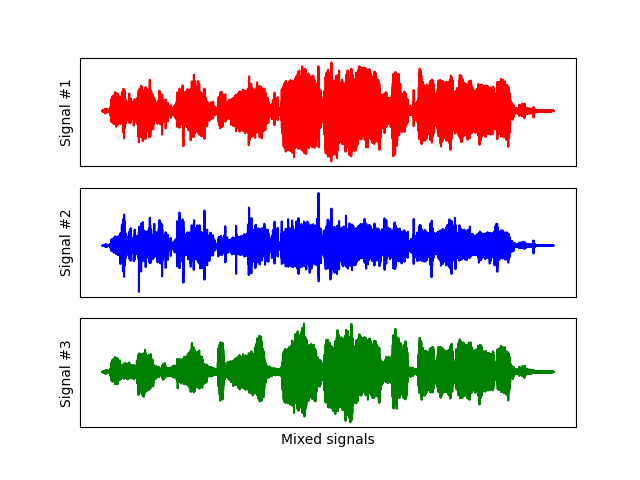
\includegraphics[width=3.6in]{mixed.png}	
	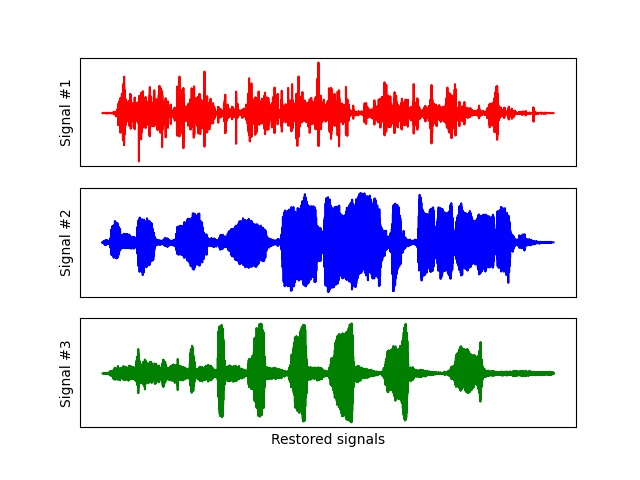
\includegraphics[width=3.6in]{restored.png}	
	\caption{Visualization of the signals: (upper) orignal signals, (middle) mixed signals, and (bottom) restored signals}
	\label{fig:signal}
\end{figure}

\begin{figure}[!t]
	\centering
	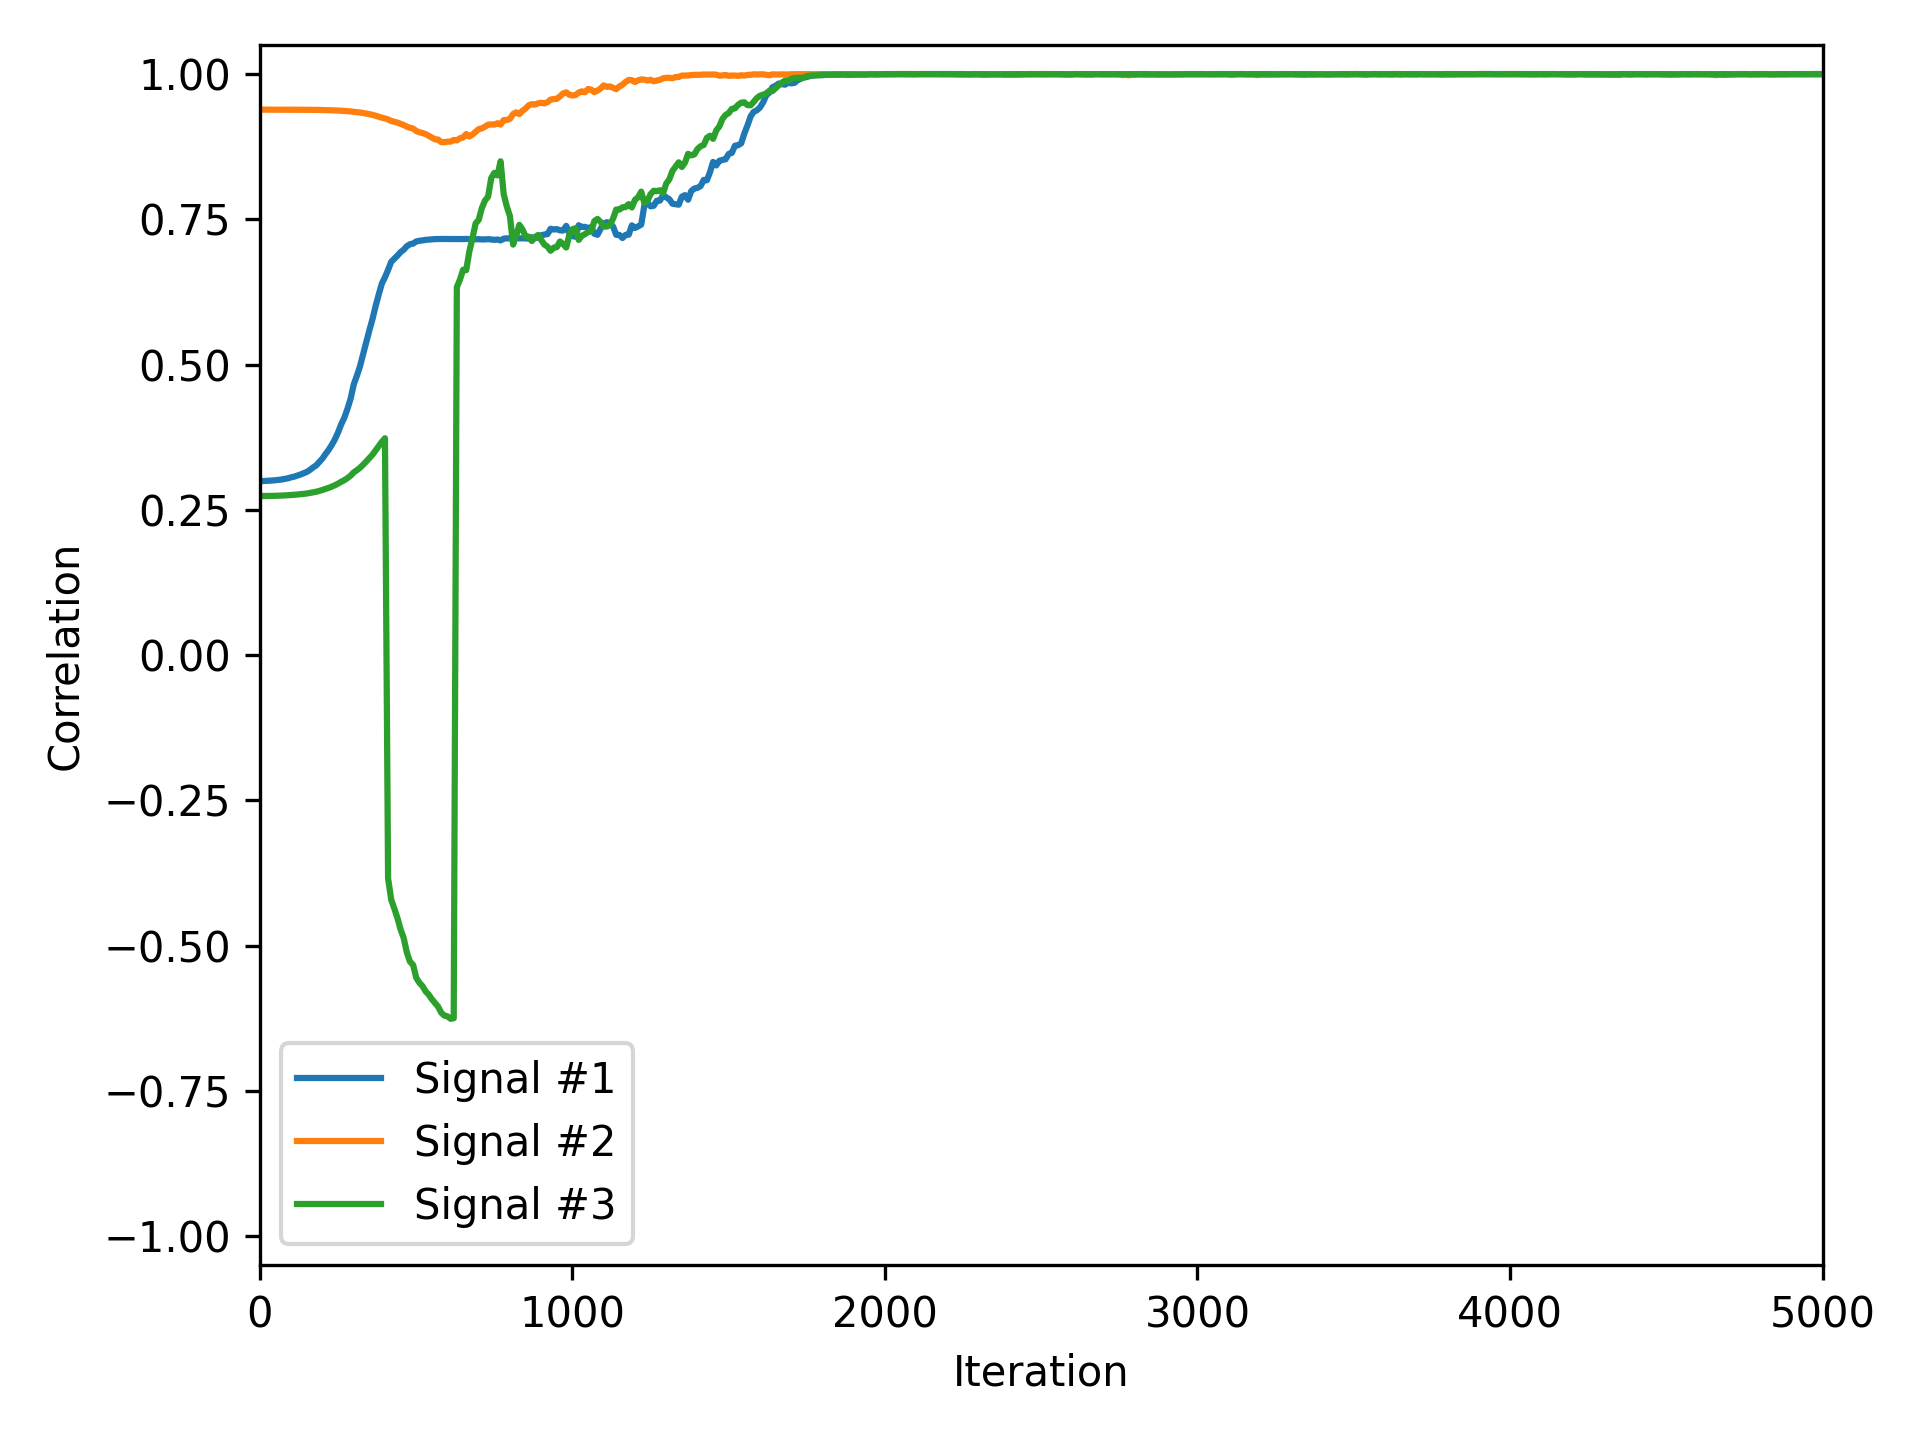
\includegraphics[width=3.6in]{basic_test.png}	
	\caption{Correlation between each source signal and the corresponding the restored signal.}
	\label{fig:basic_test}
\end{figure}

\begin{figure}[!t]
	\centering
	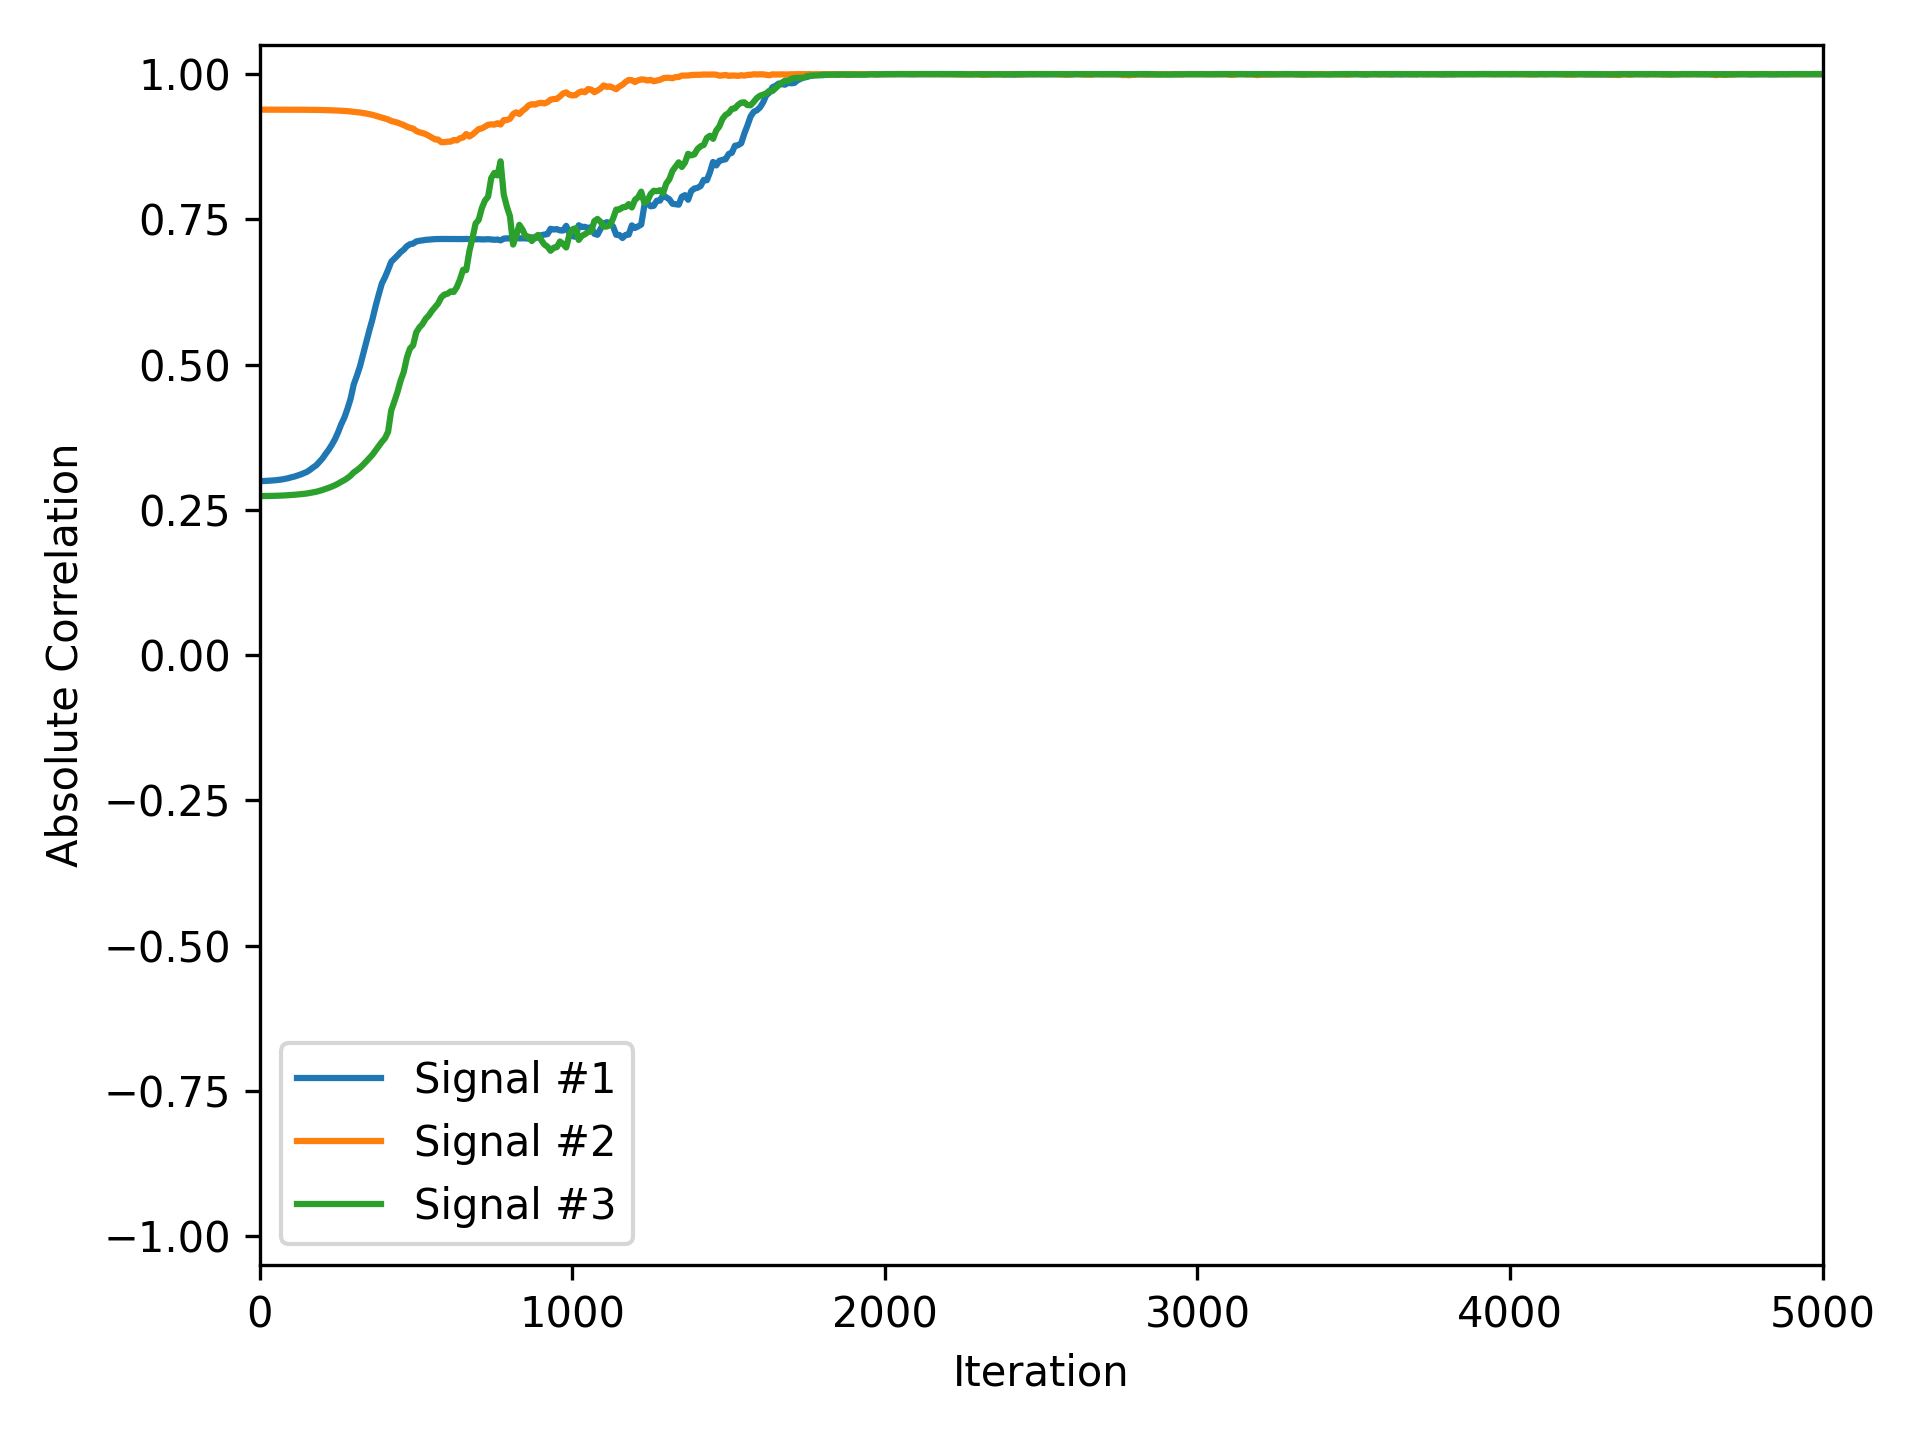
\includegraphics[width=3.6in]{basic_abs_test.png}	
	\caption{Correlation between each source signal and the corresponding the restored signal.}
	\label{fig:basic_abs_test}
\end{figure}

\subsection{Batch size}

The plot of absolute correlation at different batch sizes $t$ is presented in Fig. \ref{fig:batch_abs_test}.
In the experiment, we used $n=3$, $m=3$, $\eta=0.01$, and $k_{\text{max}} = 5000$.
From the results, we can find that the correlation increases fastest at the batch size $k=32$. In a larger batch size, there is a negligible drop at the speed of correlation magnitude increases. On the other hand, a batch size causes a significant drop, which implies that the model suffers from a lack of sample information.

\begin{figure}[!t]
	\centering
	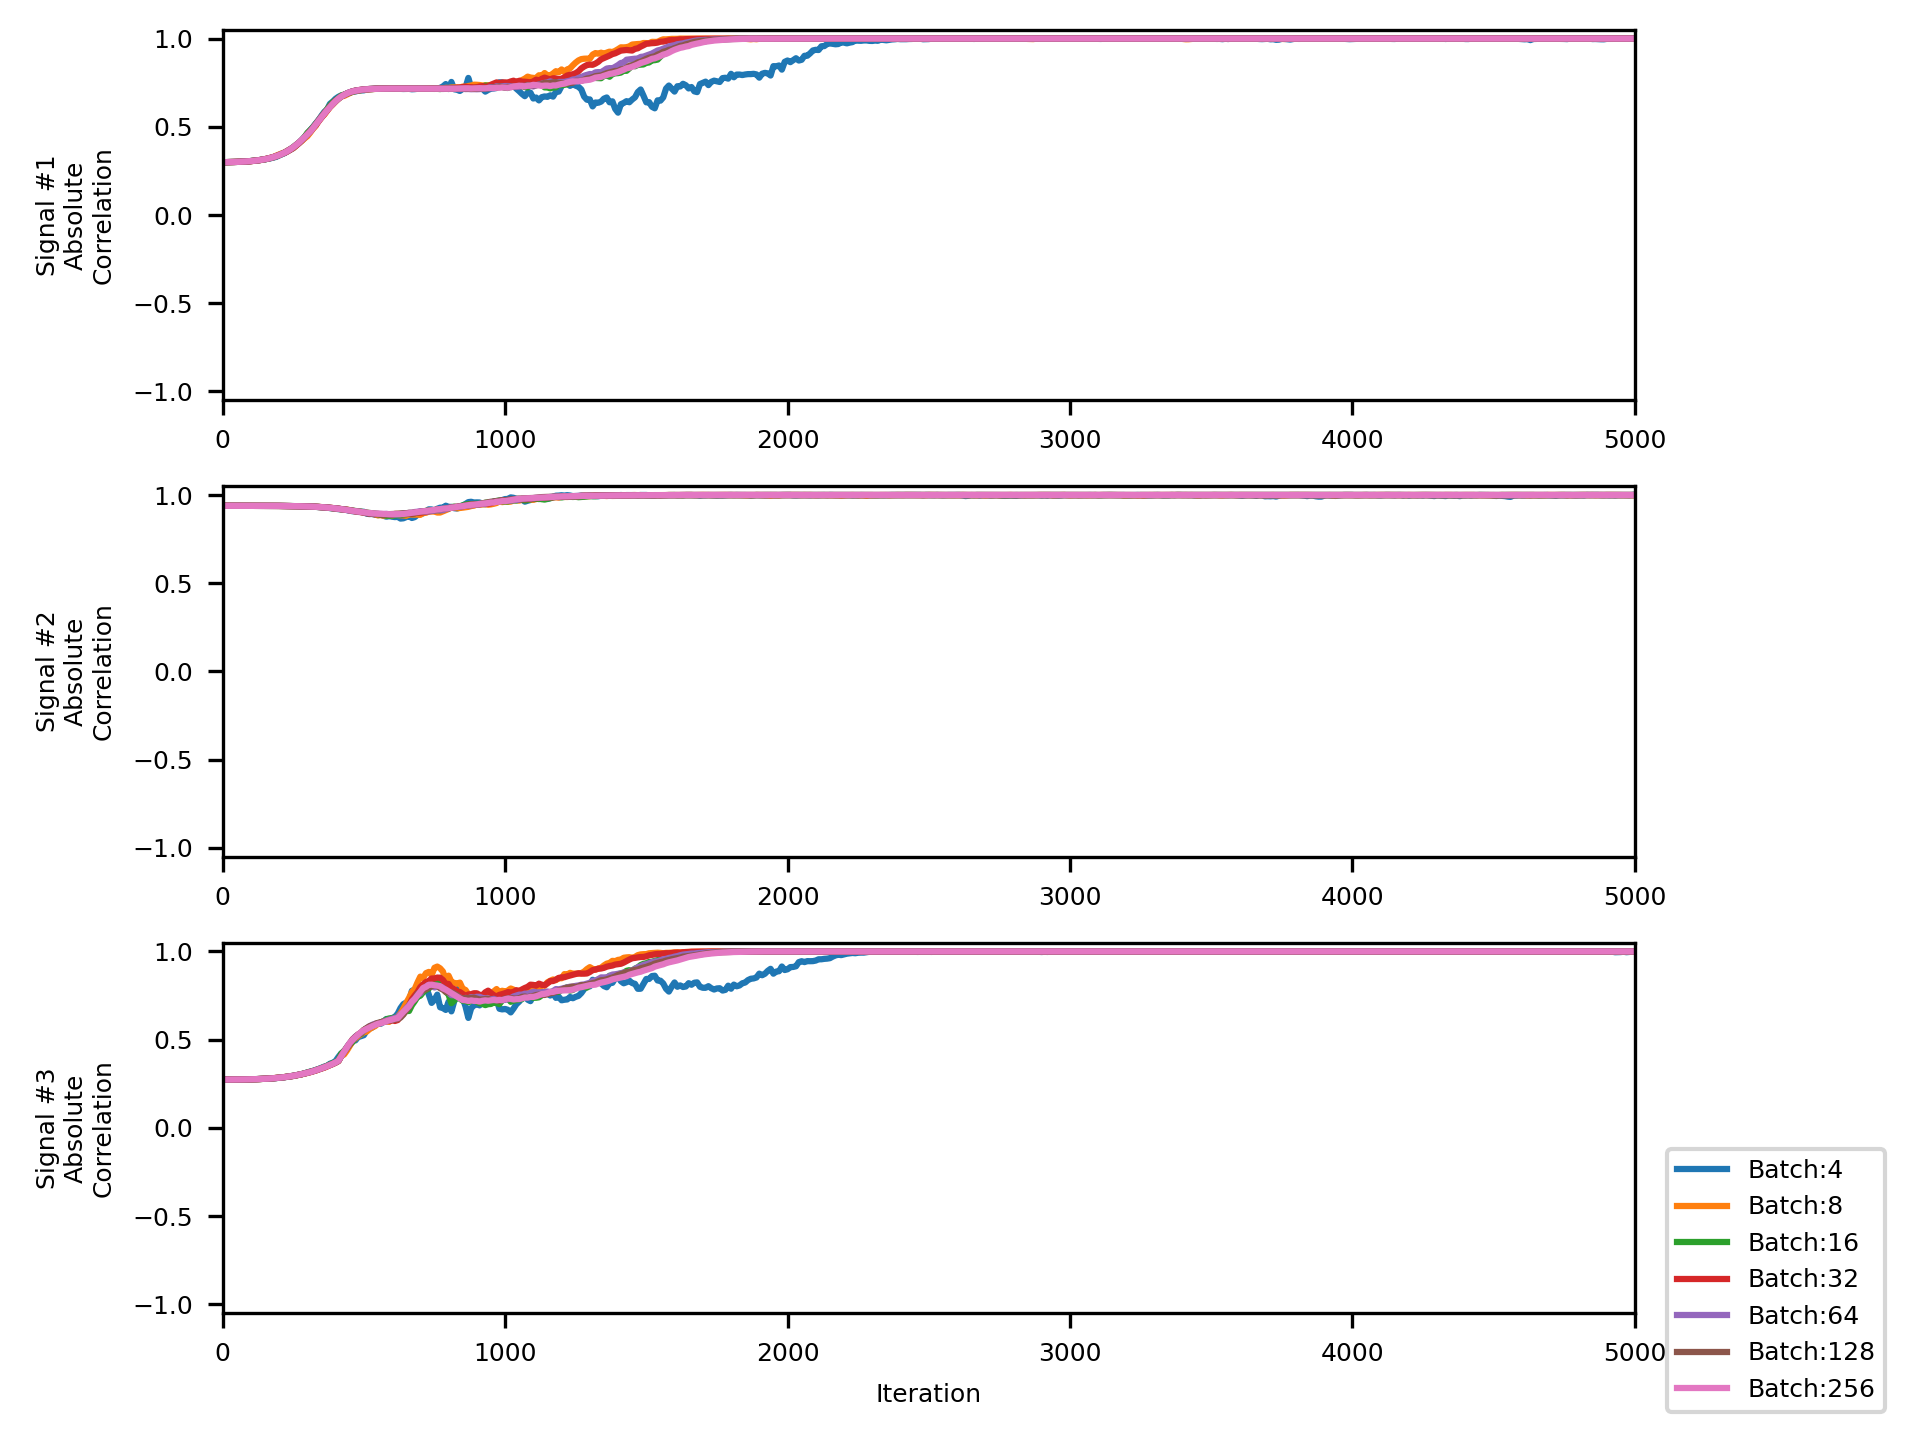
\includegraphics[width=3.6in]{batch_abs_test.png}	
	\caption{Absolute correlation changes on batch size: batch sample sizes are chosen in [4, 8, 16, 32, 64, 128, 256].}
	\label{fig:batch_abs_test}
\end{figure}


\subsection{Learning rate}

The plot of absolute correlation at different learning rates $\eta$ is presented in Fig. \ref{fig:eta_abs_test}.
In the experiment, we used $n=3$, $m=3$, $t=16$, and $k_{\text{max}} = 5000$.
From the results, we can find that a higher learning rate yields faster. However, an excessively high learning rate prevents the convergence at gradient descent, which causes unstable performance, such as perturbations in correlation remaining even after enough iterations.

\begin{figure}[!t]
	\centering
	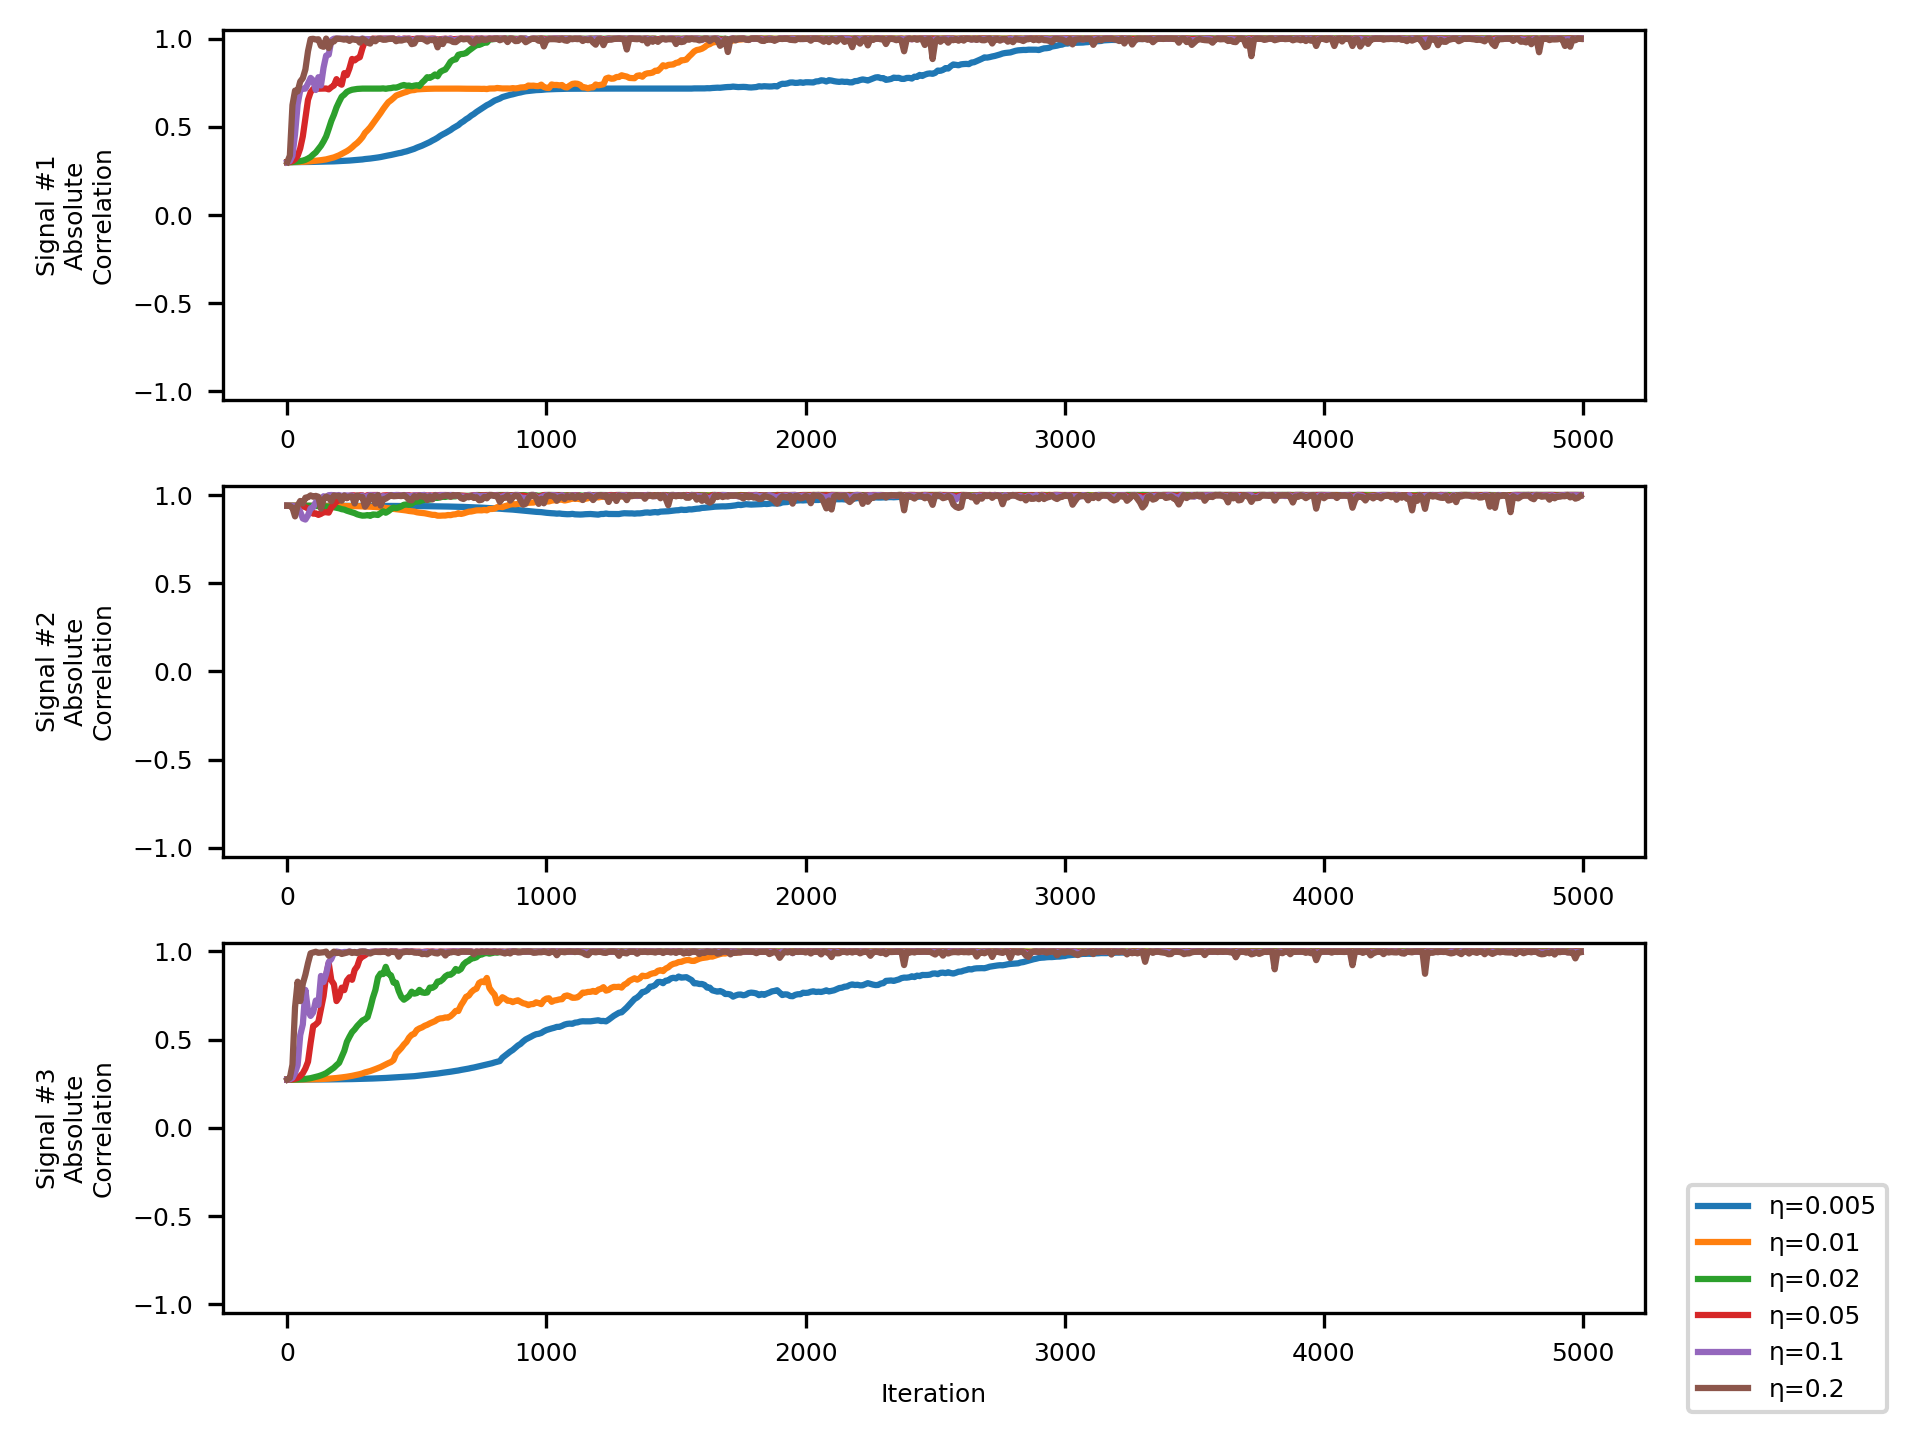
\includegraphics[width=3.6in]{eta_abs_test.png}	
	\caption{Absolute correlation changes on learning rate: learning rates are chosen in [0.005, 0.01, 0.02, 0.05, 0.1, 0.2].}
	\label{fig:eta_abs_test}
\end{figure}



\subsection{Sample size}

The plot of absolute correlation at different sample signal numbers $m$ is presented in Fig. \ref{fig:sample_abs_test}.
In the experiment, we used $n=3$, $t=16$, $\eta=0.01$, and $k_{\text{max}} = 5000$.
From the result at $m=2$, we can find that the model fails to restore Signal \#1. This implies that a smaller sample number than the given source signal number, $m<n$, causes the dimension issue at the unmixing $W$, where the model cannot fully extract the original signals.

\begin{figure}[!t]
	\centering
	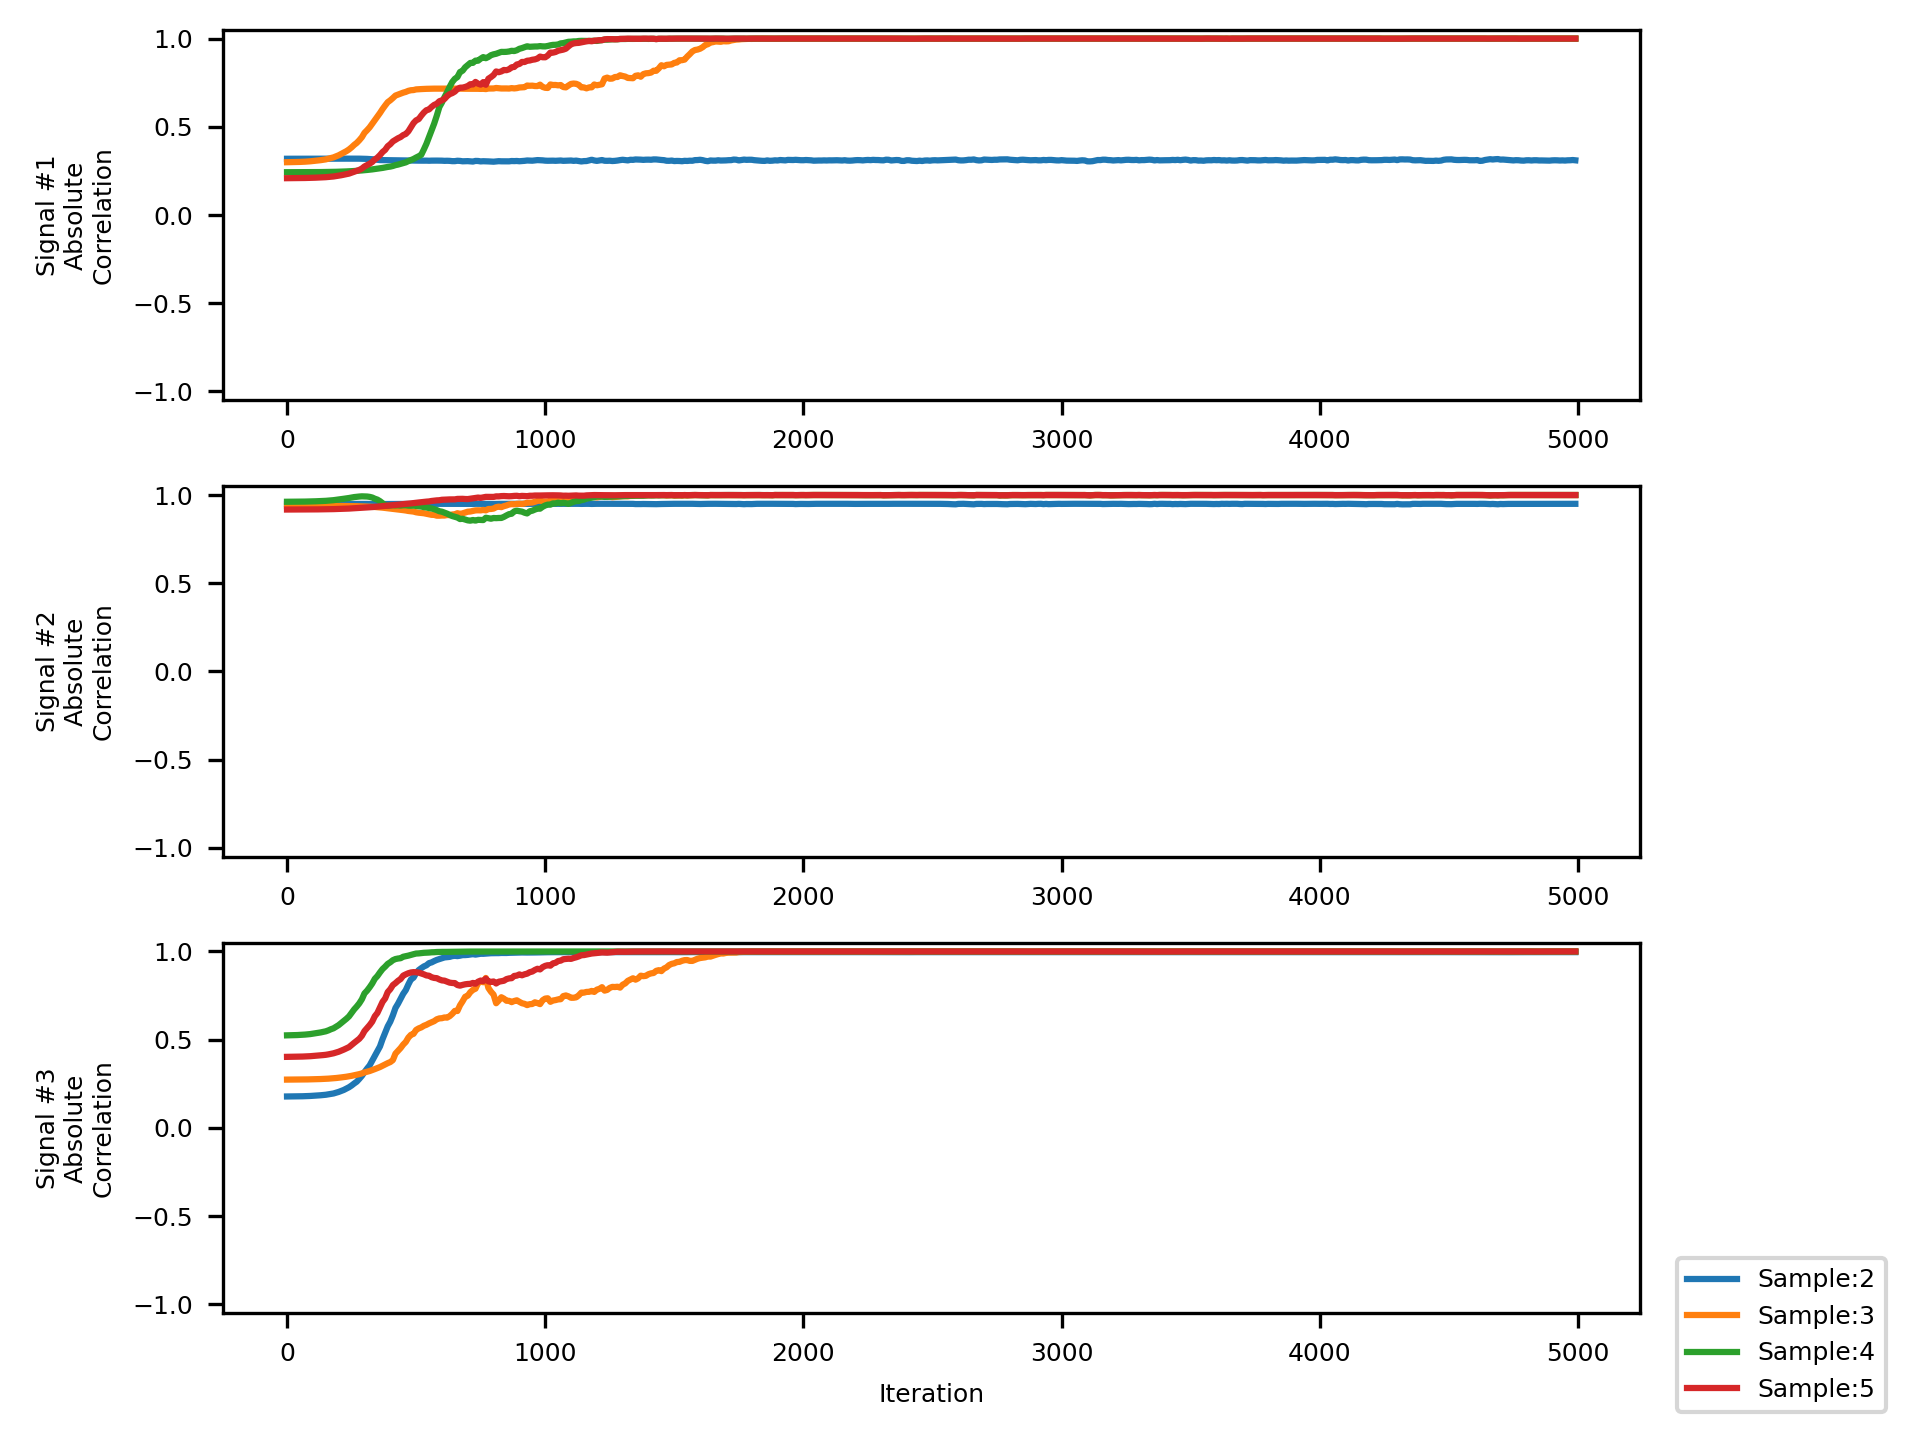
\includegraphics[width=3.6in]{sample_abs_test.png}	
	\caption{Absolute correlation changes on sample sizes: sample sizes are chosen in [2, 3, 4, 5].}
	\label{fig:sample_abs_test}
\end{figure}


\section{Summary} %Intermediate/Preliminary Results: State and evaluate your results upeto the milestone

The GP model and gradient descent for regressing the model from raw motion data are implemented in the assignment. 
For training, we mixed 5 human motion dataset of the same task demonstration and estimated the trajectory by regressing the GP model.
By the regression, we optimized the optimal set of hyperparamters for the finite GP kenel from the given data.
From the results of the experiments, we can confirmed that a sliding window kernel is able to fit the given data more accurately than a global kernel function.
This is verified by taking the mean of the log-likelihood and square errors over all the points it spans.

%\section*{Acknowledgments}

%% Use plainnat to work nicely with natbib. 

\bibliographystyle{plainnat}
\begin{thebibliography}{9}
\bibitem{bishop}
Christopher M. Bishop (2006) \emph{Pattern Recognition and Machine Learning}, Springer.
\end{thebibliography}


\end{document}


